\documentclass{article}

% Language setting
% Replace `english' with e.g. `spanish' to change the document language
\usepackage[portuguese]{babel}

% Set page size and margins
% Replace `letterpaper' with `a4paper' for UK/EU standard size
\usepackage[a4paper,top=2cm,bottom=2cm,left=2cm,right=2cm,marginparwidth=1.75cm]{geometry}

% Useful packages
\usepackage{graphicx}
\usepackage{float}

\title{Resolução de problemas como problemas de pesquisa no espaço de estados}
\author{João Matos (32409), João Rouxinol (44451) e André Rato (45517)}

\begin{document}
\maketitle

\section{Agente A até à saída S}
\subsection{O problema}
\subsubsection{Espaço de resultados}
\paragraph{} Para a representação do problema, os estados seguem todos a estrutura \textbf{"\texttt{e(C, L)}"}, em que C é o número da coluna e L o número da linha do estado. Através desta representação, foi possível criar os estados inicial e final: \texttt{estado\_inicial(e(2, 7))} e \texttt{estado\_final(e(5, 1))}.

\subsubsection{Restrições}
\paragraph{} As retrições seguem a mesma representação que os estados inicial e final, tido sido então criada uma "lista" de cláusulas:
\begin{itemize}
  \item \texttt{bloqueada(e(1, 2))}
  \item \texttt{bloqueada(e(3, 1))}
  \item \texttt{bloqueada(e(3, 2))}
  \item \texttt{bloqueada(e(4, 4))}
  \item \texttt{bloqueada(e(4, 5))}
  \item \texttt{bloqueada(e(4, 6))}
  \item \texttt{bloqueada(e(7, 2))}
\end{itemize}

\subsubsection{Operadores de transição de estado}
\paragraph{} De modo a representar as deslocações do agente para cima, baixo, esquerda e direita, o predicado \texttt{op/4} foi definido, utilizando a estrutura \texttt{op(estado\_atual, operador, estado\_seguinte, custo)}. Este predicado verifica se o movimento é válido no tamanho do problema, neste caso 7, e se a posição para qual o agente se movimenta está ou não bloqueada.

\begin{figure}[h]
\centering
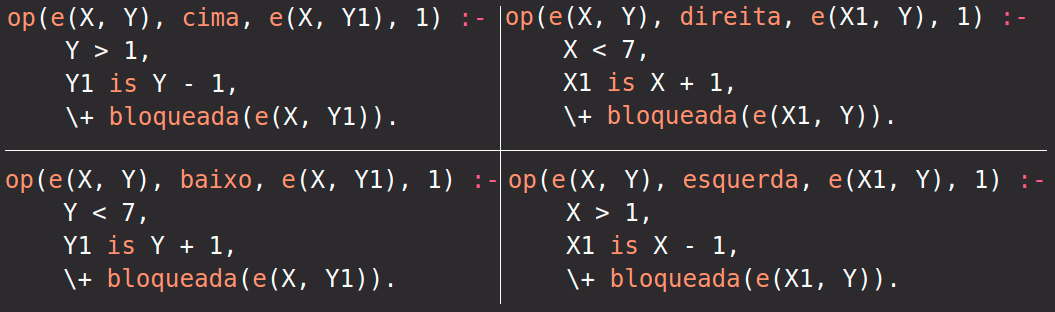
\includegraphics[width=0.8\textwidth]{operadores.png}
\caption{\label{fig:op}Operadores de transição de estado.}
\end{figure}

\subsection{Algoritmos de pesquisa não informada}
\paragraph{} A análise dos algoritmos de pesquisa não informada foi realizada com um estado inicial diferente do estado inicial do enunciado. Isto aconteceu pois devido ao elevado número de nós que necessitam de ser guardados simultanemante em memória para os algoritos de pesquisa em largura e em profundidade, é retornado o erro \texttt{global stack overflow}, informando que a memória disponibilizada para a execução do programa não é suficiente para armazenar os nós necessários. Sendo assim, o estado inicial utilizado foi \texttt{e(3, 5)}, não sendo alterado o estado final.
\subsubsection{Análise dos algoritmos}
\begin{table}[h]
\centering
\begin{tabular}{l|c|c|c|c}
Algoritmo & Estados Visitados & Estados em Memória & Profundidade & Custo \\\hline
Largura & 1045 & 1187 & 6 & 6 \\\hline
Profundidade & 13 & 12 & 6 & 6 \\\hline
Profundidade Iterativa & 56812 & 14 & 6 & 6 
\end{tabular}
\caption{\label{tab:pni}Análise dos algoritmos de pesquisa não informada.}
\end{table}

\subsubsection{Algoritmo mais eficiente}
\paragraph{} Analisando os valores obtidos para os três algoritmos de pesquisa não informada, é possível constatar que:
\begin{itemize}
  \item a \textbf{pesquisa em profundidade} possui menor número de estados visitados;
  \item a \textbf{pesquisa  em profundidade} possui menor número de estados em memória;
  \item todos os algoritmos encontram uma solução para o problema à mesma profundidade e com o mesmo custo.
\end{itemize}
\paragraph{} Após a análise acima, pode verificar-se que, embora o algoritmo de pesquisa em largura ser um algoritmo de pesquisa completo, este necessita de utilizar muita memória para guardar todos os nós. A pesquisa em profundidade iterativa é também um algoritmo completo, mas necessita de incrementar a profundidade a cada passo e refazer todas as árvores dos passos anteriores. Assim, mesmo não obtendo uma solução ótima, escolhe-se o algoritmo de pesquisa em profundidade.

\subsubsection{Código em Prolog}
\begin{verbatim}
    pesquisa_profundidade([no(E,Pai,Op,C,P)|_],no(E,Pai,Op,C,P)):-
        inc,
        estado_final(E).
    pesquisa_profundidade([E|R],Sol):-
        inc,
        expande(E,Lseg),
        insere_fim(R,Lseg,Resto),
        length(Resto,N),
        actmax(N),
        pesquisa_profundidade(Resto,Sol).
\end{verbatim}

\subsection{Heurísitcas}
\subsubsection{Distância de Manhattan}
\paragraph{} Como primeira heurística, foi utilizada a distância de Manhattan: $d((x1, y1), (x2, y2)) = |x1 - x2| + |y1 - y2|$.

\begin{figure}[h]
\centering
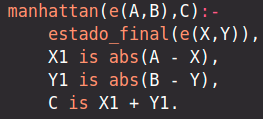
\includegraphics[width=0.3\textwidth]{manhattan.png}
\caption{\label{fig:man}Implementação da distância de Manhattan em Prolog.}
\end{figure}

\subsubsection{Distância euclidiana}
\paragraph{} Já a segunda heurística escolhida foi a distância euclidiana: $d((x1, y1), (x2, y2)) = \sqrt{(x1-x2)^2 + (y1-y2)^2}$.

\begin{figure}[h]
\centering
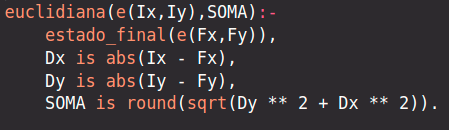
\includegraphics[width=0.5\textwidth]{euclidiana.png}
\caption{\label{fig:euc}Implementação da distância euclidiana em Prolog.}
\end{figure}

\subsection{Algoritmos de pesquisa informada}
\paragraph{} A análise dos algoritmos de pesquisa informada foi realizada utilizando os estads inicial e final do enunciado.

\subsubsection{Análise dos algoritmos}

\begin{table}[H]
\centering
\begin{tabular}{l|c|c|c|c}
Algoritmo de Pesquisa & Estados Visitados & Estados em Memória & Profundidade & Custo \\\hline
A* com dist. de Manhattan & 60 & 43 & 9 & 9 \\\hline
A* com dist. euclidiana & 66 & 39 & 9 & 9 \\\hline
Ansiosa com dist. de Manhattan & 11 & 14 & 9 & 9 \\\hline
Ansiosa com dist. euclidiana & 11 & 15 & 9 & 9 
\end{tabular}
\caption{\label{tab:pni}Análise dos algoritmos de pesquisa informada.}
\end{table}

\subsubsection{Algoritmo mais eficiente}
\paragraph{} Analisando os valores obtidos para os três algoritmos de pesquisa informada, é possível constatar que:
\begin{itemize}
  \item a \textbf{pesquisa ansiosa}, com qualqur uma das duas heurísticas, possui menor número de estados visitados;
  \item a \textbf{pesquisa ansiosa}, que utiliza como heurística a distância de Manhattan, possui menor número de estados em memória;
  \item todos os algoritmos encontram uma soluç̃ao para o problema à mesma profundidade e com o mesmo custo.
\end{itemize}

\paragraph{} Após a análise acima, pode verificar-se que o algoritmo com melhor desempenho foi o algoritmo de pesquisa ansiosa, sendo que o algoritmo que utiliza a distância de Manhattan necessitava de menos estados em memória para chegar à solução. Verificamos também que a pesquisa ansiosa expande o nó que aparenta estar mais próximo do estado final, o que neste caso, acaba por melhorar o desempenho do algoritmo.

\subsubsection{Código em Prolog}
\begin{verbatim}
    pesquisa_g([no(E,Pai,Op,C,HC,P)|_],no(E,Pai,Op,C,HC,P)):-
        estado_final(E).
    pesquisa_g([E|R],Sol):- 
        inc, 
        asserta(fechado(E)), 
        expande_g(E,Lseg),
        insere_ord(Lseg,R,Resto),
        length(Resto,N),
        actmax(N),
        pesquisa_g(Resto,Sol).
\end{verbatim}

\newpage

\section{Agente A empurra a caixa C até à saída S}
\subsection{O problema}
\subsubsection{Espaço de resultados}
\paragraph{} Para a representação do problema, os estados seguem todos a estrutura \textbf{"\texttt{p(C1, L1, C2, L2)}"}, em que C1 é o número da coluna e L1 o número da linha em que se encontra o agente e C2 é o número da coluna e L2 o número da linha em que se encontra a caixa. Através desta representação, foi possível criar os estados inicial e final: \texttt{estado\_inicial(p(2, 7, 2, 6))} e \texttt{estado\_final(p(\_, \_, 5, 1))}.

\subsubsection{Restrições}
\paragraph{} As retrições seguem a mesma representação que o problema anterior e que os estados inicial e final, tido sido então criada uma "lista" de cláusulas:
\begin{itemize}
  \item \texttt{bloqueada(p(1, 2))}
  \item \texttt{bloqueada(p(3, 1))}
  \item \texttt{bloqueada(p(3, 2))}
  \item \texttt{bloqueada(p(4, 4))}
  \item \texttt{bloqueada(p(4, 5))}
  \item \texttt{bloqueada(p(4, 6))}
  \item \texttt{bloqueada(p(7, 2))}
\end{itemize}

\subsubsection{Operadores de transição de estado}
\paragraph{} De modo a representar as deslocações do agente para cima, baixo, esquerda e direita, e o movimento da caixa, o predicado \texttt{op/4} foi definido, utilizando a estrutura \texttt{op(estado\_atual, operador, estado\_seguinte, custo)}.

\begin{figure}[h]
\centering
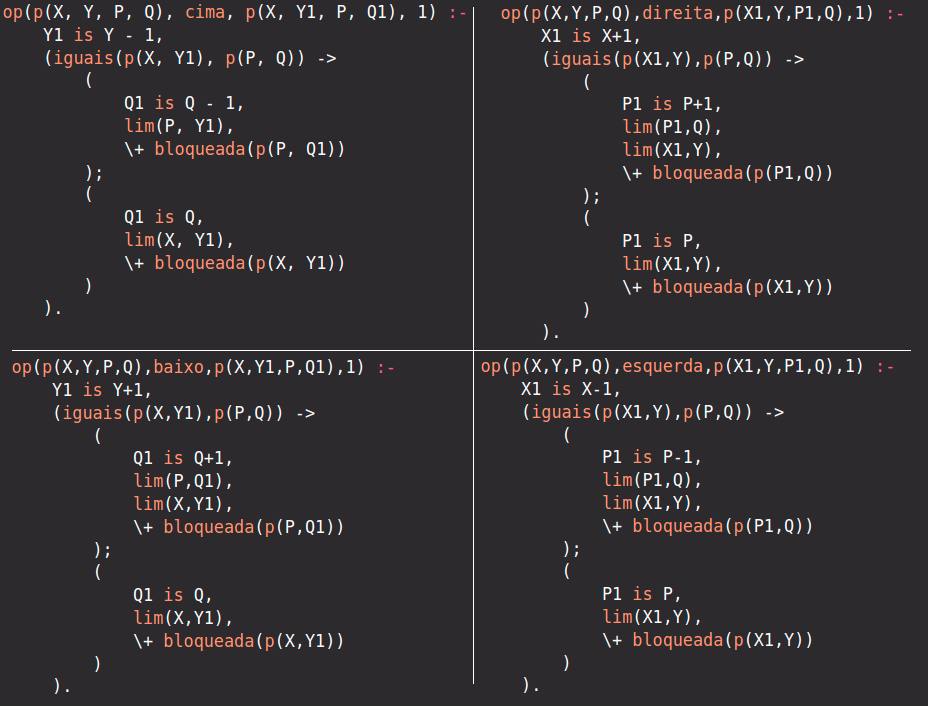
\includegraphics[width=0.8\textwidth]{pi.png}
\caption{\label{fig:op}Operadores de transição de estado.}
\end{figure}

\subsection{Algoritmos de pesquisa não informada}
\paragraph{} A análise dos algoritmos de pesquisa não informada foi realizada com um estado inicial diferente do estado inicial do enunciado. Isto aconteceu pois devido ao elevado número de nós que necessitam de ser guardados simultanemante em memória para os algoritos de pesquisa em largura e em profundidade, é retornado o erro \texttt{global stack overflow}, informando que a memória disponibilizada para a execução do programa não é suficiente para armazenar os nós necessários. Sendo assim, o estado inicial utilizado foi \texttt{p(5, 7, 5, 6)}, não sendo alterado o estado final.
\subsubsection{Análise dos algoritmos}
\begin{table}[h]
\centering
\begin{tabular}{l|c|c|c|c}
Algoritmo & Estados Visitados & Estados em Memória & Profundidade & Custo \\\hline
Largura & 213 & 216 & 5 & 5 \\\hline
Profundidade & 11 & 12 & 5 & 5 \\\hline
Profundidade Iterativa & 6281 & 12 & 5 & 5 
\end{tabular}
\caption{\label{tab:pni}Análise dos algoritmos de pesquisa não informada.}
\end{table}

\subsubsection{Algoritmo mais eficiente}
\paragraph{} Analisando os valores obtidos para os três algoritmos de pesquisa não informada, é possível constatar várias coisas:
\begin{itemize}
  \item a \textbf{pesquisa em profundidade} possui menor número de estados visitados;
  \item as \textbf{pesquisas em profudidade} e \texttt{em profundidade iterativa} possuem menor número de estados em memória;
  \item todos os algoritmos encontram uma soluç̃ao para o problema à mesma profundidade e com o mesmo custo.
\end{itemize}

\paragraph{} Após a análise acima, pode verificar-se que o algoritmo com melhor desempenho foi, novamente, o algoritmo de pesquisa em profundidade. No entanto, é possível afirmar-se que o algoritmo de pesquisa em profundidade iterativa tem um grande nível de abrangência no que toca à gestão da memória disponibilizada, sendo, dos três algoritmos, aquele que guarda simultaneante, menos estados em meória.

\subsubsection{Código em Prolog}
\begin{verbatim}
    pesquisa_profundidade([no(E,Pai,Op,C,P)|_],no(E,Pai,Op,C,P)):-
        inc,
        estado_final(E).
    pesquisa_profundidade([E|R],Sol):-
        inc,
        expande(E,Lseg),
        insere_fim(R,Lseg,Resto),
        length(Resto,N),
        actmax(N),
        pesquisa_profundidade(Resto,Sol).
\end{verbatim}

\subsection{Heurísitcas}
\subsubsection{Distância de Manhattan entre a caixa C e a saída S - heurística 1}
\paragraph{} Como primeira heurística, foi utilizada a distância de Manhattan entre as posições da caixa C e da saída S: $d((x1, y1), (x2, y2)) = |x1 - x2| + |y1 - y2|$.

\begin{figure}[h]
\centering
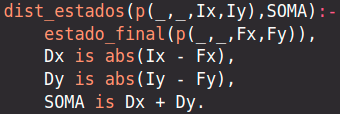
\includegraphics[width=0.3\textwidth]{estados.png}
\caption{\label{fig:man}Implementação da distância de Manhattan entre a caixa C e a saída S em Prolog.}
\end{figure}

\newpage

\subsubsection{Diferença entre as linhas da caixa C e a saída C - heurística 2}
\paragraph{} Já a segunda heurística escolhida foi a diferença entre o valor da linha de C e o valor da linha de S: $d((x1, y1), (x2, y2)) = |y1 - y2|$.

\begin{figure}[h]
\centering
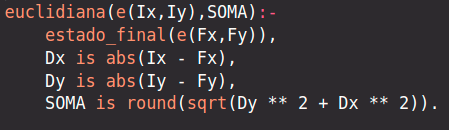
\includegraphics[width=0.4\textwidth]{euclidiana.png}
\caption{\label{fig:euc}Implementação da distância euclidiana em Prolog.}
\end{figure}

\subsection{Algoritmos de pesquisa informada}
\paragraph{} A análise dos algoritmos de pesquisa informada foi realizada utilizando os estads inicial e final do enunciado.
\subsubsection{Análise dos algoritmos}

\begin{table}[h]
\centering
\begin{tabular}{l|c|c|c|c}
Algoritmo de Pesquisa & Estados Visitados & Estados em Memória & Profundidade & Custo \\\hline
A* com heurística 1 & 1203 & 459 & 16 & 16 \\\hline
A* com heurística 2 & 2305 & 513 & 16 & 16 \\\hline
Ansiosa com heurística 1 & 467 & 54 & 16 & 16 \\\hline
Ansiosa com heurística 2 & 2097 & 198 & 16 & 16 
\end{tabular}
\caption{\label{tab:pni}Análise dos algoritmos de pesquisa informada.}
\end{table}

\subsubsection{Algoritmo mais eficiente}
\paragraph{} Analisando os valores obtidos para os três algoritmos de pesquisa informada, é possível constatar que:
\begin{itemize}
  \item a \textbf{pesquisa ansiosa com a heurística 1} possui menor número de estados visitados;
  \item a \textbf{pesquisa ansiosa com a heurística 1} possui menor número de estados em memória;
  \item todos os algoritmos encontram uma soluç̃ao para o problema à mesma profundidade e com o mesmo custo.
\end{itemize}

\paragraph{} Podemos então dizer que o melhor algoritmo de pesquisa informada para este problema é o algoritmo de pesquisa ansiosa em que a heurística utilizada é a distâcia de Manhattan entre a caixa C e a saída S, mostrando ter um melhor desempenho geral, não visitando tantos nós, nem utilizando tanto memória como os demais algoritmos.

\subsubsection{Código em Prolog}
\begin{verbatim}
    pesquisa_g([no(E,Pai,Op,C,HC,P)|_],no(E,Pai,Op,C,HC,P)):-
        estado_final(E).
    pesquisa_g([E|R],Sol):- 
        inc, 
        asserta(fechado(E)), 
        expande_g(E,Lseg),
        insere_ord(Lseg,R,Resto),
        length(Resto,N),
        actmax(N),
        pesquisa_g(Resto,Sol).
\end{verbatim}

 \newpage
 
\section{Executar pesquisas}
\paragraph{} Para executar o programa basta:
\begin{itemize}
  \item carregar o problema desejado e o tipo de pesquisa que é pretendido ("pi", para pesquisas informadas, ou "pni", para pesquisas não informadas, utilizando \texttt{[<problema>, <tipo\_pesquisa>].};
  \item chamar o predicado responśavel pela pesquisa, utilizando \texttt{pesquisa(<problema>, <algoritmo>).};
  \item esperar que o programa encontre a solução para o problema pretendido e observar os resultados obtidos.
\end{itemize}
\end{document}